%%-------------------------------------------------------------------------------------- Início
\begin{frame}[allowframebreaks, t, fragile]{Ação: New}
	\begin{figure}[h!]
		\centering
		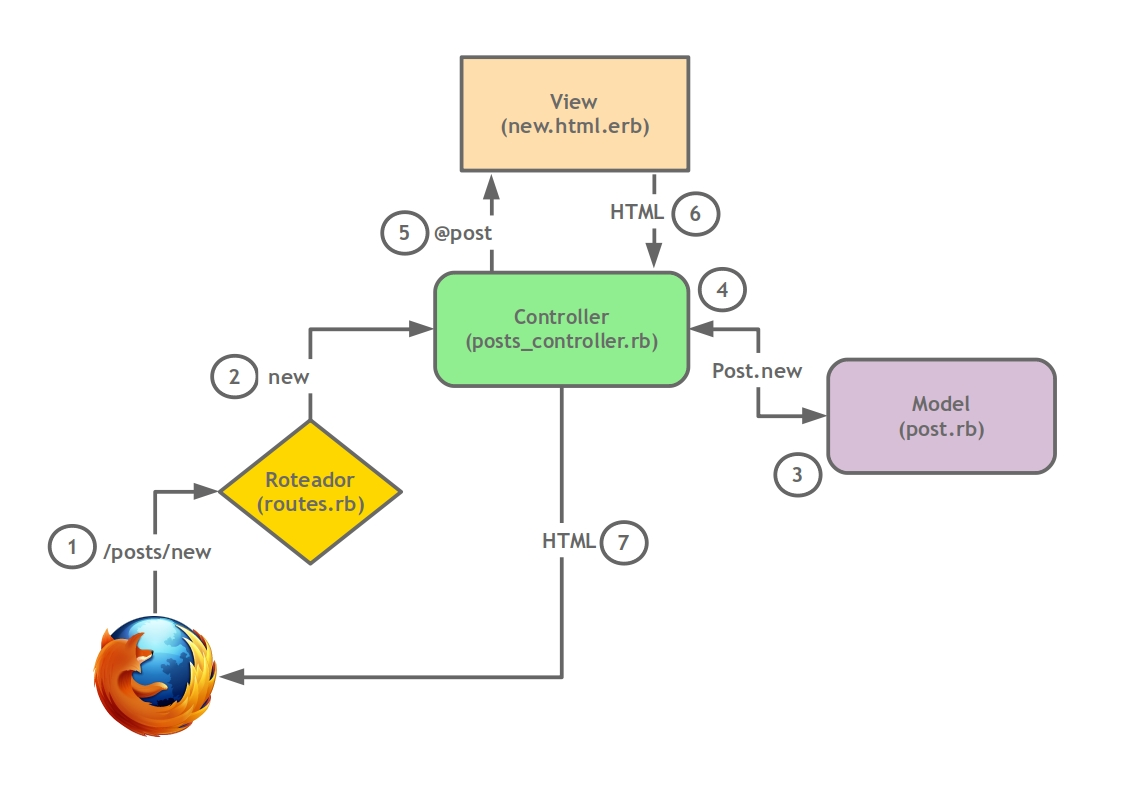
\includegraphics[width=0.75\textwidth]{imagens/mvc-action-new.jpg}
	\end{figure}
	\framebreak
	\begin{itemize}
		\item Um novo objeto \alert{@post} da classe \alert{Post} é instanciado 
		\item Procura pela visão \alert{new.html.erb} para renderizar a resposta
		\begin{lstlisting}[style=RubyInputStyle, caption=app/controllers/posts\_controller.rb]
Class PostsController < ApplicationController
  def new
    @post = Post.new 
  end 
end
		\end{lstlisting}
	\end{itemize}
\end{frame}

\begin{frame}[allowframebreaks, t, fragile]{Visão: New}
	\begin{itemize}
		\item Reinicie o servidor web e acesse a url \url{http:\\localhost:3000/posts/new}. Veja o erro que ocorreu.
		\item Implemente a visão \alert{new.html.erb}:
		\begin{lstlisting}[style=RubyInputStyle, caption=views/posts/new.html.erb]
<h1>Novo Post</h1>
<%= form_with model: @post, local: true do |form| %>
	<p>
		<%= form.label :title %><br>
		<%= form.text_field :title %>
	</p>
	
	<p>
		<%= form.label :body %><br>
		<%= form.text_area :body %>
	</p>
	
	<p>
		<%= form.submit %>
	</p>
<% end %>	
		\end{lstlisting}
	\end{itemize}	
\end{frame}